
\section{Experimentation}
\label{sec:experiments}
In this section we examine the properties of \SCAMPLON{} and 
compare them to the properties of \CYCLON{}, a state-of-the-art cyclic peer sampling service.
As \CYCLON{} uses a fixed-sized partial view, we optimize it for a network of 1000 peers.
As shown in this paper\cite{erdos1959random}
To optimize it for said network size, the partial view size $c$ is set to $7\approx \ln{1000}$
while in each cycle we exchange $l=3$ peers.
The experiments\footnote{Implementation: https://github.com/anonymous/anonymous4now}
involve up to 100,000 nodes and are carried out on \PEERSIM{} \cite{peersim}, 
a simulator for peer-to-peer networks.
We define a cycle as $\Delta t$ in which each peer has executed its active protocol once.

We inspect three properties characteristic for random graphs, 
the \emph{average shortest path length}, the \emph{average clustering coefficient},
and \emph{the partial view size distribution}. Additionally, we investigate on
\emph{robustness to random failures}.

\subsection{Clustering coefficient}

\begin{figure}
    \centering
    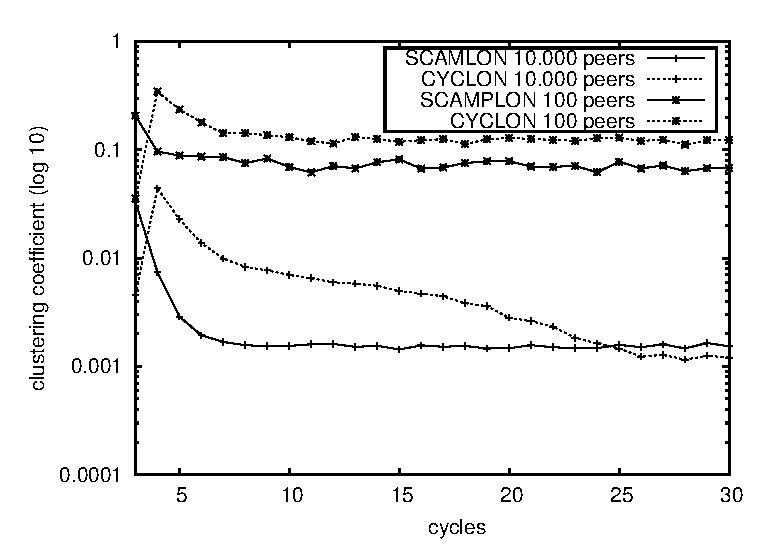
\includegraphics[width=0.49\textwidth]{img/cluster.eps}
    \caption{Clustering coefficient}
    \label{fig:clustering}
\end{figure}


\begin{asparadesc}
\item[Objective:]
    %% Highlight  
    We want to evaluate to what degree \SCAMPLON{} generates clusters in the overlay.
    To satisfy the random peer sampling objective it is desired that the network has very few clusters,
    thus has a low clustering coefficient.
\item[Description:] 
    The average clustering coefficient $\overline{C}$  measures the connectivity of each peer's neighborhood in the network.
  \begin{equation}
    \overline{C} = {1\over |\mathcal{N}|}\sum\limits_{x\in\mathcal{N}}C_x
    \end{equation}
    where $C_x$ is the local clustering coefficient of Peer $p_x$. The higher
    the coefficient, the more likely the network contains cliques. 
    The experiments involve 100, 1000, 10000 and 100000 peers. 


\item[Results:]



\item[Reasons:]

    

\end{asparadesc}



\subsection{Average path length}

\begin{figure}
    \centering
    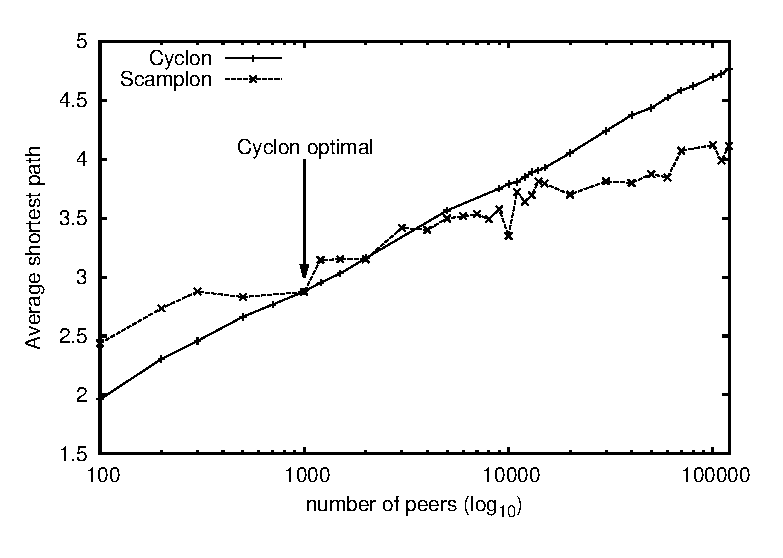
\includegraphics[width=0.49\textwidth]{img/avgpath.eps}
    \caption{Average shortest path}
    \label{fig:avgpath}
\end{figure}

\begin{asparadesc}
\item[Objective:] 
    For messages to disseminate quickly into the network it is crucial 
    that the shortest path to other peers is, in fact, short.
\item[Description:] The average path length is the average of the shortest path
  length between peers in the graph. It counts the minimum number of hops to
  reach a peer from another given peer.
  For performance reasons, we selected a subset of 7 nodes, calculated their
  average shortest path and averaged it.
\item[Results:]
When undersized, \CYCLON{} yield a shorter average shortest path then \SCAMPLON{}~\ref{fig:clustering}.
\item[Reasons:]
\end{asparadesc}

\subsection{Partial view size distribution}

\subsection{Resilience to failure}

\subsection{Churn}

\begin{figure}
    \centering
    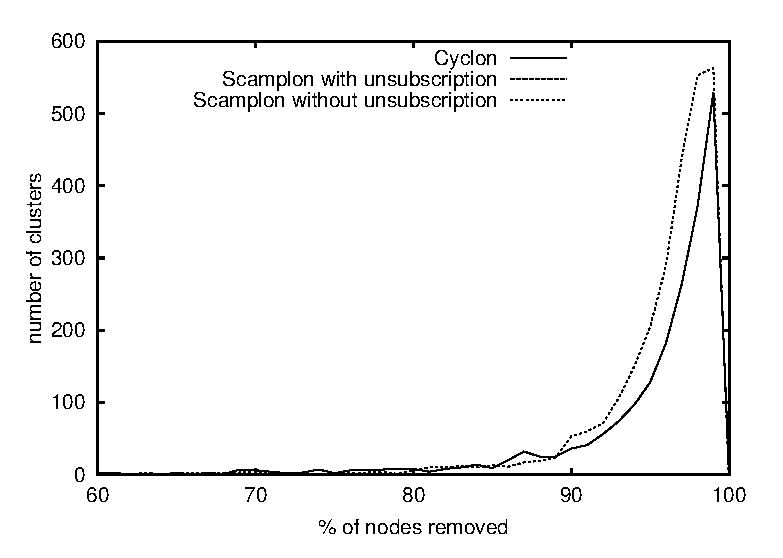
\includegraphics[width=0.49\textwidth]{img/churn.eps}
    \caption{Churn}
    \label{fig:churn}
\end{figure}

\begin{algorithm}

\small
\algrenewcommand{\algorithmiccomment}[1]{\hskip2em$\rhd$ #1}

\newcommand{\comment}[1]{$\rhd$ #1}

\algblockdefx[initially]{initially}{endInitially}
  [0] {\textbf{INITIALLY:}}

\algblockdefx[pas]{pas}{endPas}
  [0] {\textbf{EVENTS:}}

\newcommand{\LINEFOR}[2]{%
  \algorithmicfor\ {#1}\ \algorithmicdo\ {#2} %
  }

\newcommand{\LINEIFTHEN}[2]{%
  \algorithmicif\ {#1}\ \algorithmicthen\ {#2} %
  }

\newcommand{\INDSTATE}[1][1]{\State\hspace{\algorithmicindent}}

\begin{algorithmic}[1]
  \Statex
  \initially
  \State $\mathcal{I}$ \hfill \label{line:inview}
  \comment{set of peers targeting us ($p$) in their partial view}
  \endInitially

  \pas
    \Function{unSubscribe}{\ }
    \For{$i\leftarrow 0$ \textbf{to} $min(|\mathcal{P}|,\, |\mathcal{P}|-1)$ 
      \label{line:bridge}}    
    \State \textbf{let} $\langle n,\,\_ \,\rangle \leftarrow \mathcal{P}[i]$;
    \State $sendTo(\, \mathcal{I}[\,i\%|\mathcal{I}|\,],\, 'unSubs',\, n)$;
    \EndFor
    \EndFunction
    \Statex
    \Function{onUnSubs}{$o, \, n$} 
    \hfill \comment{$o$: origin; $n$: neighbor to add}
    \State $\mathcal{P}\leftarrow (\mathcal{P}\setminus o)
    \uplus\{\langle n,\,0\rangle\}$;
    \EndFunction
  \endPas
\end{algorithmic}

\caption{\label{algo:unsubscription}Unsubscription protocol from
  SCAMP~\cite{ganesh2003peer}}
\end{algorithm}

\subsection{Synthesis}

%%% Local Variables:
%%% mode: latex
%%% TeX-master: "../paper"
%%% End:
